
% ==============================================================================
% START: Abstract
% ==============================================================================

\begin{abstract}
   This document intents to give theoretical support and context to the built application
   \href{https://github.com/gariciodaro/arXiv-haystack-app}{arXiv-haystack-app}. Using 
   \href{https://www.kaggle.com/Cornell-University/arxiv}{Arxiv} and Neural Information Processing 
    Systems (\href{https://www.kaggle.com/benhamner/nips-papers}{NIPS}) datasets I created
    a relational database model that allows the user to do Ad-Hoc queries for analytics. Using \href{https://github.com/deepset-ai/haystack}{haystack}  the application allows for question and answering on user defined abstracts of the database. 


\begin{figure}[h]
\centering
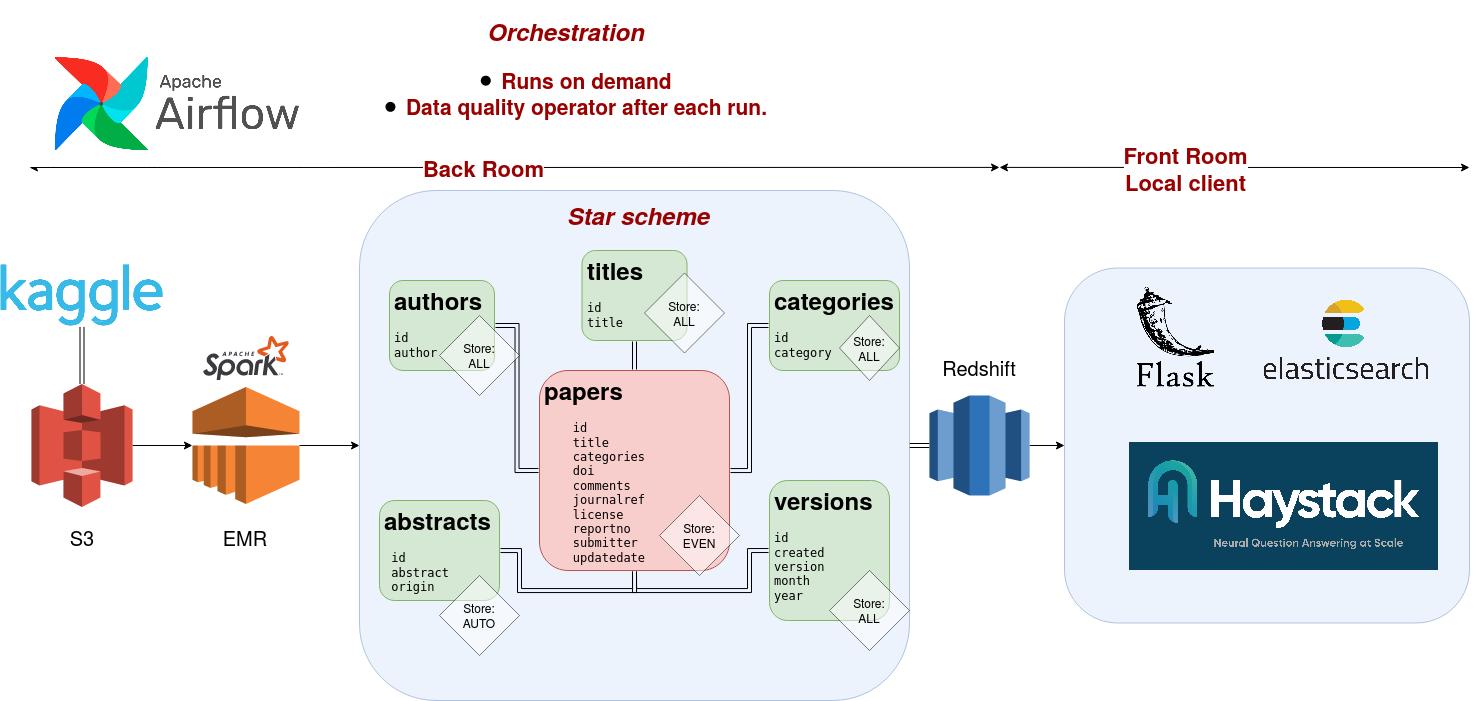
\includegraphics[width=1\linewidth]{images/architecture}
\caption{Project Architecture}
\label{fig:architecture}
\end{figure}

\end{abstract}\hspace{10pt}

\keywords{S3, Amazon Elastic MapReduce, Pyspark, Airflow, Redshift, Flask, NLP, Q\&A, Haystack, Machine Learning, Full stack development, Data Engineering.}
% ==============================================================================x
% END: Abstract
% ==============================================================================